\chapter{File System}

\section{Size of file cache}
In this part, we try to determine the file cache size.

\paragraph{Methodology}
If the file the fit into cache totally, then it would be very fast to read. If the file is too big that can not be put into cache totally, then read would be slower then that fir into cache totally. 

So I prepared 40 files with different sizes ranging from 1GB to 4GB. We read each file 10 times and calculate  read cycles/MB.

\paragraph{Predictions}
Our computer main memory is 8GB. So the cache must be less than 8GB; Besides, the project web page says it is a notable fraction of main memory and can be several GBs. So we predict it is 2GBs.

\paragraph{Results}
We present our measure results. By the way, we did not show the results of files that are less than 3GB, we have run them and narrow down 
narrow the range from 3GB to 4GB. So we only include result from 3GB to 4GB here.

\begin{center}
\begin{tabular}{l*{6}{c}r}
File Size             &  Cycles/MB\\
\hline
3000MB & 610 \\
3100MB & 614 \\
3200MB & 598 \\
3300MB & 622 \\
3400MB & 1965 \\
3500MB & 5498 \\
3600MB & 5572 \\
3700MB & 5503 \\
3800MB & 5673 \\
3900MB & 5657 \\
4000MB & 5598 \\

\end{tabular}
\end{center}

\begin{figure}[htbp] %  figure placement: here, top, bottom, or page
   \centering
   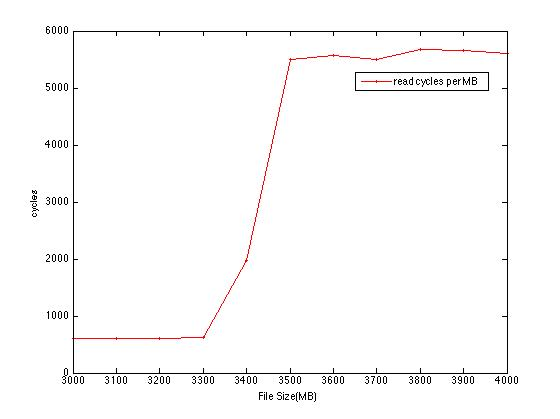
\includegraphics[width=5in]{./pics/41.jpg} 
   \caption{read cycles}
   \label{fig:read cycles}
\end{figure}

\paragraph{Discussion}
The graph shows that the file cache size is between 3300MB and 3500MB. Before this experiment, I did not realize that OS will use so many spaces for file cache. This optimization speed up file reading time significantly. I do this measurement when my computer is free. If my computer are running many applications that consume many memory, then I think OS could not provide so much memory for file caching.

\section{File read time}
In this part, we report for both sequential and random access as a function of file size.

\paragraph{Methodology}
First, in order not to measure cached data, we want to set O\_DIRECT flag when opening a file, which could minimize cache effects of the I/O from this file. But Mac OS does not support O\_DIRECT. So we looked through Apple document and find we can set F\_NOCACHE flag in fcntl().

Besides, we use read() for sequential access, because read() will modify file pointer that fit the situation; However for random access it is bad to use read(), because we have to use lseek() to move the file pointer to target position which will significantly cost time. So we use pread() instead of read() for random access. Pread() works just like read() but reads from the specified position in the file without modifying the file pointer.

We provide several files with different sizes and iterate 100 times, then calculate  the average per-block read time.

\paragraph{Predictions}
Because we are using SSD, the speed of sequential and random access may be very similar to each other. Considering that we did not use file cache, we will fetch each block of data from disk. So I predict the speed is 19000 cycles per blocks, plus 1000 cycles for software.

\paragraph{Results}
We present our measure results. The base file is 4KB, and we define log(4KB) = 2.

\begin{figure}[htbp] %  figure placement: here, top, bottom, or page
   \centering
   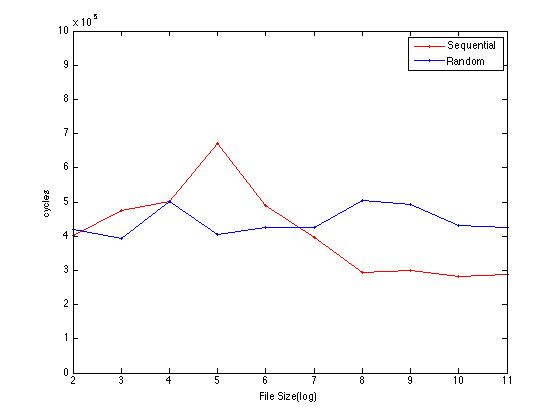
\includegraphics[width=5in]{./pics/42.jpg} 
   \caption{read cycles per block}
   \label{fig:read cycles per block}
\end{figure}

\begin{center}
\begin{tabular}{| p{2cm} | p{2.5cm} | p{2.5cm} | p{2.5cm} | p{2.5cm} | p{3cm}}
File Size &  Base Hardware Performance  & Estimated Software Overhead  & Predicted Time  & Measured Time & Std  \\

\hline
4KB & 19000 cycles& 1000 cycles& 20000 cycles& 401481 cycles & 10665 cycles \\ 
8KB & 19000 cycles& 1000 cycles& 20000 cycles& 475677 cycles & 13289 cycles \\ 
16KB & 19000 cycles& 1000 cycles& 20000 cycles& 501356 cycles & 10032 cycles \\
32KB & 19000 cycles& 1000 cycles& 20000 cycles& 670260 cycles & 15723 cycles \\
64KB & 19000 cycles& 1000 cycles& 20000 cycles& 489722 cycles & 12875 cycles \\
128KB & 19000 cycles& 1000 cycles& 20000 cycles& 397495 cycles & 12200 cycles \\
256KB & 19000 cycles& 1000 cycles& 20000 cycles& 293712 cycles & 9200 cycles \\
512KB & 19000 cycles& 1000 cycles& 20000 cycles& 300106 cycles &  10085 cycles \\
1024KB & 19000 cycles& 1000 cycles& 20000 cycles& 281106 cycles & 5602 cycles \\
2048KB & 19000 cycles& 1000 cycles& 20000 cycles& 287629 cycles & 6001 cycles \\

\end{tabular}
\end{center}

Above is the result of sequential access. We can see on average it takes about 300000-600000 cycles to read each file block, far exceeding than we predicted previously.

\begin{center}
\begin{tabular}{| p{2cm} | p{2.5cm} | p{2.5cm} | p{2.5cm} | p{2.5cm} | p{3cm} }
File Size   & Base Hardware Performance  & Estimated Software Overhead  & Predicted Time  & Measured Time  & Std \\
\hline
4KB & 19000 cycles& 1000 cycles& 20000 cycles& 420067 cycles & 17352 cycles\\ 
8KB & 19000 cycles& 1000 cycles& 20000 cycles& 393597 cycles & 13847 cycles\\ 
16KB & 19000 cycles& 1000 cycles& 20000 cycles& 502322 cycles & 15555 cycles\\
32KB & 19000 cycles& 1000 cycles& 20000 cycles& 405538 cycles & 14200 cycles\\
64KB & 19000 cycles& 1000 cycles& 20000 cycles& 425528 cycles & 12222 cycles\\
128KB & 19000 cycles& 1000 cycles& 20000 cycles& 426442 cycles & 13902 cycles \\
256KB & 19000 cycles& 1000 cycles& 20000 cycles& 504624 cycles & 10002 cycles\\
512KB & 19000 cycles& 1000 cycles& 20000 cycles& 492654 cycles & 12320 cycles \\
1024KB & 19000 cycles& 1000 cycles& 20000 cycles& 430804 cycles & 10800 cycles\\
2048KB & 19000 cycles& 1000 cycles& 20000 cycles& 426658 cycles & 9602 cycles \\

\end{tabular}
\end{center}

Above is the result of random access. We can see on average it takes about 400000-500000 cycles to read each file block, far exceeding than we predicted previously.

\paragraph{Discussion}
As we have predicted, random access is almost as fast as sequential access due to SSD. But we predict cycles wrongly. Without file cache, it would be very expensive to do file reading. Each block would cost almost 300000-600000 cycles on average.

Then I remove F\_NOCACHE flag to do file reading, finding that it only takes about 1000-2000 cycles per block, which is so cheap compared with no cache. It speeds up over 100 times. So, in most situations open file with cache is good for program performance.

As for "sequential" access might not be sequential, we have to seek the next right position for sequential read without cache. Because contents in a file may not be consecutive.

\section{Remote file read time}
In this section, we conduct the previous experiment for a remote file system.

\paragraph{Methodology}
We use the same method described in previous section. The only difference is that we now read a remote file. Note, page size in that machine is 8KB.

\paragraph{Predictions}
The remote machine use SSD, and the network bandwidth is 1000Mb/s, these two machines are in same LAN. So the effect of network may not seem so obvious.

Based on the results of previous section, we add 20\% overhead in hardware and software. Don't forget that the pagesize now is 8KB. And we think sequential access time is close to random access time. 

\paragraph{Results}

We present our measure results. The base file is 4KB, and we define log(4KB) = 2.

\begin{figure}[htbp] %  figure placement: here, top, bottom, or page
   \centering
   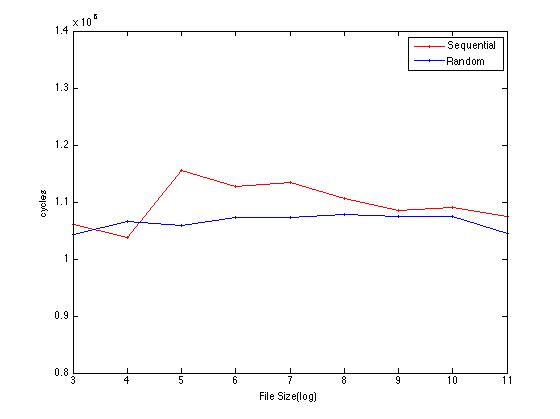
\includegraphics[width=4in]{./pics/43.jpg} 
   \caption{remote read cycles per block}
   \label{fig:remote read cycles per block}
\end{figure}

\begin{center}
\begin{tabular}{| p{2cm} | p{2.5cm} | p{2.5cm} | p{2.5cm} | p{2.5cm} | p{3cm} }
File Size  & Base Hardware Performance  & Estimated Software Overhead  & Predicted Time  & Measured Time  & Std \\
\hline
8KB & 800000 cycles& 10000 cycles& 810000 cycles& 1060023 cycles & 12040 cycles \\ 
16KB & 800000 cycles& 10000 cycles& 810000 cycles& 1037613 cycles & 11025 cycles\\ 
32KB & 800000 cycles& 10000 cycles& 810000 cycles& 1155908 cycles & 20301 cycles\\
64KB & 800000 cycles& 10000 cycles& 810000 cycles& 1127454 cycles & 18750 cycles\\
128KB & 800000 cycles& 10000 cycles& 810000 cycles& 1134455 cycles & 23004 cycle \\
256KB & 800000 cycles& 10000 cycles& 810000 cycles& 1105819 cycles & 13334 cycle \\
512KB & 800000 cycles& 10000 cycles& 810000 cycles& 1085479 cycles & 17648 cycles\\
1024KB & 800000 cycles& 10000 cycles& 810000 cycles& 1089600 cycles & 20334 cycles\\
2048KB & 800000 cycles& 10000 cycles& 810000 cycles& 1074542 cycles & 17778 cycles \\

\end{tabular}
\end{center}

Above is the result of sequential access.

\begin{center}
\begin{tabular}{| p{2cm} | p{2.5cm} | p{2.5cm} | p{2.5cm} | p{2.5cm} | p{3cm} }
File Size  & Base Hardware Performance  & Estimated Software Overhead  & Predicted Time  & Measured Time  & Std \\
\hline
8KB & 800000 cycles& 10000 cycles& 810000 cycles& 1043427 cycles & 9400 cycles\\ 
16KB & 800000 cycles& 10000 cycles& 810000 cycles& 1065662 cycles & 13298 cycles\\ 
32KB & 800000 cycles& 10000 cycles& 810000 cycles& 1058558 cycles & 12201 cycles\\
64KB & 800000 cycles& 10000 cycles& 810000 cycles& 1073499 cycles & 16652 cycles\\
128KB & 800000 cycles& 10000 cycles& 810000 cycles& 1073262 cycles & 8553 cycles\\
256KB & 800000 cycles& 10000 cycles& 810000 cycles& 1077349 cycles & 8890 cycles\\
512KB & 800000 cycles& 10000 cycles& 810000 cycles& 1074041 cycles & 13009 cycles\\
1024KB & 800000 cycles& 10000 cycles& 810000 cycles& 1074543 cycles & 10004 cycles\\
2048KB & 800000 cycles& 10000 cycles& 810000 cycles& 1044684 cycles & 9330 cycles\\

\end{tabular}
\end{center}

Above is the result of random access.

\paragraph{Discussion}
Due to previous experience, this time our estimation is very close to the measured results. And it seems that the overhead is not so much compared with file cache. If one machine is in China, another one is in US, maybe network is very expensive compared to other factors.

SSDs also make random access as fast as sequential access.

\paragraph{Question} What is the "network penalty" of accessing files over the network?  As we have predicted, compared with file cache, the network overhead is about 20\%, around 200000 cycles.

\section{Contention}
In this section, we report the average time to read one file system block of data as a function of the number of processes simultaneously performing the same operation on different files on the same disk (and not in the file buffer cache).

\paragraph{Methodology}
As previous experiment, we continue using F\_NOCACHE flag to disable file cache. In this experiment, we create several processes. Each process read different file which is of the same size : 1MB. And we iterate 100 times to get average data. 

\paragraph{Predictions}
We are sure that the more process number, the more cycles it spend on reading file. We think each read will result in a context switch to another process. We present predictions with results in the following table. We use 1MB file, including 256 blocks. Based on previous experiment on sequential reading 1MB file, when there is only 1 process, the reading cycles are 281106. When increasing a process, we add about 15000 cycles for hardware and 1000 for software.

\paragraph{Results}
We present our measure results.

\begin{center}
\begin{tabular}{| p{2cm} | p{2.5cm} | p{2.5cm} | p{2.5cm} | p{2.5cm} |  p{3cm}}
nprocesses   & Base Hardware Performance  & Estimated Software Overhead  & Predicted Time  & Measured Time  & Std \\
\hline
1 & 280000 cycles& 1000 cycles& 281000cycles & 229003 cycles & 8572 cycles \\
2 & 295000 cycles& 2000 cycles& 297000 cycles& 253880 cycles & 9400 cycles \\
3 & 310000 cycles& 3000 cycles& 313000 cycles& 209028 cycles & 9210 cycles \\
4 & 325000 cycles& 4000 cycles& 329000 cycles& 240578 cycles & 10450 cycles \\
5 & 340000 cycles& 5000 cycles& 345000 cycles& 432147 cycles & 8322 cycles \\
6 & 355000 cycles& 6000 cycles& 371000 cycles& 438801 cycles & 9726 cycles \\
7 & 370000 cycles& 7000 cycles& 377000 cycles& 459831 cycles & 8625 cycles \\
8 & 385000 cycles& 8000 cycles& 393000 cycles& 415745 cycles & 13392 cycles \\
9 & 400000 cycles& 9000 cycles& 409000 cycles& 474147 cycles & 12209 cycles \\
10 & 415000 cycles& 10000 cycles& 425000 cycles& 491004 cycles & 7490 cycles \\
11 & 430000 cycles& 11000 cycles& 441000 cycles& 515341 cycles & 15526 cycles \\
12 & 445000 cycles& 12000 cycles& 457000 cycles& 515871 cycles & 10024 cycles\\
13 & 460000 cycles& 13000 cycles& 473000 cycles& 536629 cycles & 20047 cycles \\
14 & 475000 cycles& 14000 cycles& 489000 cycles& 568728 cycles & 14478 cycles \\
15 & 490000 cycles& 15000 cycles& 505000 cycles& 590147 cycles & 25980 cycles \\

\end{tabular}
\end{center}

\begin{figure}[htbp] %  figure placement: here, top, bottom, or page
   \centering
   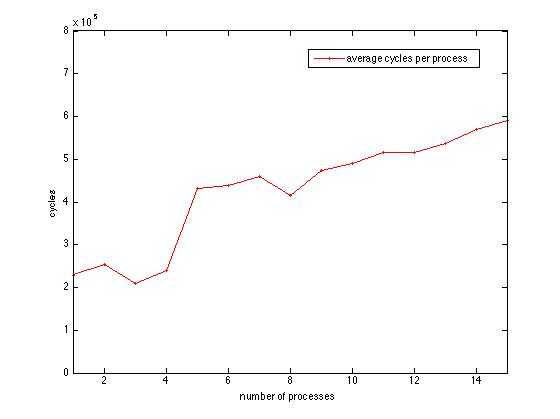
\includegraphics[width=4.5in]{./pics/44.jpg} 
   \caption{average cycles per process}
   \label{fig:average cycles per process}
\end{figure}

\paragraph{Discussion}
We can see that generally, with the increasing of process, the average cycle increase too. 

Our prediction is so close to the measured results. I am very surprised, I had thought that the measured results may exceed millions of cycles due to context switch between processes.

When I set the file cache flag, the cycles reduce to about 6000-8000 per block.

If we use HDD, each read will take many seek time. Now we use SSD, the cost is very small. That's the big difference between SSD and HDD.